\documentclass{article}
\NeedsTeXFormat{LaTeX2e}
\RequirePackage{amsmath}                % Mathematics
\RequirePackage{amssymb}                % Symbols
\RequirePackage{amsfonts}               % Fonts
\RequirePackage[table]{xcolor}          % Using colours in documents
\RequirePackage{tabularx}               % Additional functions to tables
\RequirePackage{booktabs}               % Adds more line functionality to tables
\RequirePackage{epigraph}               % Allow comments on the Part page
\RequirePackage{multirow}               % Counterpart of multi columns
\RequirePackage{enumitem}               % Customise the list spacing
\RequirePackage{geometry}               % Document geometry
\RequirePackage{titlesec}               % Custom titles
\RequirePackage{titletoc}               % Custom table of contents
\RequirePackage{fancyhdr}               % Custom header/footer
\RequirePackage{graphicx}               % Adding images
\RequirePackage{float}                  % Additional float parameters
\RequirePackage{tikz}                   % Create graphic elements
\RequirePackage{datetime}               % Used in preface for monthname
\RequirePackage[final]{microtype}       % Refinements towards typographical perfection
\RequirePackage[nottoc]{tocbibind}      % Add the lists to the table of contents
\RequirePackage{xspace}                 % Ensures correct spacing after macros like \deg
\RequirePackage{etoolbox}               % General toolbox (e.g. \ifdefvoid)
\RequirePackage{pdfpages}               % Insert pdfs
\RequirePackage{afterpage}              % Commands after pagebreak
\RequirePackage{mathtools}              % Extension to amsmath
\RequirePackage{mathdots}               % Adds vdots, iddots, etc
\RequirePackage{wrapfig}                % Wrap figures around text
\RequirePackage{pifont}                 % Extra symbols
\RequirePackage{nomencl}                % Nomenclature
\RequirePackage{neuralnetwork}          % Neural Networks.
\RequirePackage{physics}                % Physics symbols like grad,
\RequirePackage{booktabs}               % Pretty and simple tables
\RequirePackage{colortbl}               % Coloring tables
\RequirePackage{xspace}
\RequirePackage{bm}
\RequirePackage{bbm}
\RequirePackage{multicol}
\RequirePackage{tkz-euclide}
% \RequirePackage{subfig}
\RequirePackage{subcaption}
\RequirePackage{pgfplots}
\RequirePackage{mathrsfs}
\RequirePackage{svg}
\RequirePackage{bigfoot}

% Packages with options
\RequirePackage[hidelinks]{hyperref}    % Improved referencing/links
\RequirePackage[capitalise]{cleveref}
\usepackage[linesnumbered,ruled,vlined]{algorithm2e}
\RequirePackage[sorting=none, maxbibnames=1, isbn=false]{biblatex}

\pgfplotsset{compat=newest}

% Load the tikz libraries
\usetikzlibrary{
    calc,
    shapes.misc,
    shapes.geometric,
    arrows,
    arrows.meta,
    fit,
    positioning,
    shapes.symbols,
    chains,
    mindmap,
    decorations.pathmorphing,
    decorations.markings,
    patterns,
    backgrounds,
    intersections,
}

%% Set up page geometry and margins
\geometry{
    a4paper,
    hscale=0.9,
    vscale=0.9
}


\usepackage{svg}
\usepackage{stmaryrd}
\let\svmathbb\mathbb
\renewcommand{\mathbb}[1]{\svmathbb{#1}}

\usepackage{todonotes}

\captionsetup[subfigure]{skip=0.2\baselineskip}
\captionsetup[figure]{skip=0.5\baselineskip}

% \newcommand{\tw}[]{\todo[inline, color=white]}


\usepackage{oplotsymbl}
\usepackage{relsize}
\usepackage{tikz-network}

\usetikzlibrary{external}
\tikzexternalize % activate!

\newcommand{\mat}[1]{\mathbf{#1}} % For matrices
\newcommand{\tensor}[1]{\mathcal{#1}} % For tensors
\newcommand{\vect}[1]{\mathbf{#1}} % For vectors

\begin{document}

\begin{equation}
    \centering
    \begin{tikzpicture}[baseline={-0.5*height("$=$")}]
        \Vertex[color=white, label=$\mathcal{X}$]{A}

        \Vertex[x=-1.4, Pseudo]{C}
        \Vertex[x=-1, y=-1, Pseudo]{D}
        \Vertex[y=-1.4, Pseudo]{Z}
        \Vertex[x=1, y=-1, Pseudo]{E}
        \Vertex[x=1, y=1, Pseudo]{F}

        \Edge[label=$i_1$, position={left=1mm}, color=black](A)(C)
        \Edge[label=$i_2$, position={below left=1mm}, color=black](A)(D)
        \Text[x=0.0, y=-0.5, fontsize=\tiny]{$\cdots$}
        \Edge[label=$i_N$, position={below right=1mm}, color=black](A)(E)
    \end{tikzpicture}
    = \mathcal{X} \in \mathbb{R}^{I_1 \times I_2 \times \cdots \times I_N}
    \label{fig:tnd_tensor_definition}
\end{equation}

\begin{equation}
    \centering
    \begin{tikzpicture}[baseline={-0.5*height("$=$")}]
        \Vertex[color=white, label=$\mathcal{X}$]{A}

        \Vertex[x=-1.4, Pseudo]{C}
        \Vertex[x=-1, y=-1, Pseudo]{D}
        \Vertex[y=-1.4, Pseudo]{Z}
        \Vertex[x=1, y=-1, Pseudo]{E}
        \Vertex[x=1, y=1, Pseudo]{F}

        \Edge[label=$i_1$, position={left=1mm}, color=black](A)(C)
        \Edge[label=$i_2$, position={below left=1mm}, color=black](A)(D)
        \Text[x=0.0, y=-0.5, fontsize=\tiny]{$\cdots$}
        \Edge[label=$i_N$, position={below right=1mm}, color=black](A)(E)
    \end{tikzpicture}
    \approx
    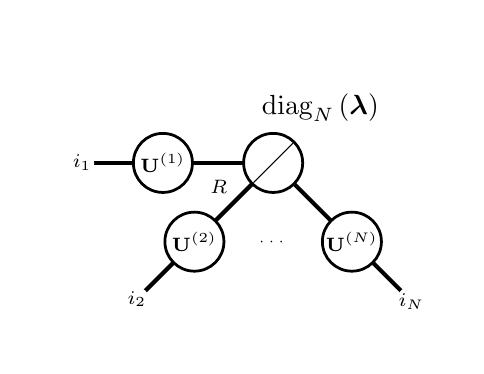
\begin{tikzpicture}[baseline={([yshift=-.5ex]current bounding box.center)}]
        \Vertex[color=white, size=0.75]{A}
        \draw (A) ++(-0.25,-0.25) -- ++(0.5,0.5); % Adjust the line as needed
        \Text[x=0.6, y=0.7]{$\operatorname{diag}_N\left(\boldsymbol{\lambda } \right)$}

        \Vertex[x=-1.4, color=white, size=0.75, label=$\mathbf{U}^{(1)}$]{B}
        \Vertex[x=-1, y=-1, color=white, size=0.75, label=$\mathbf{U}^{(2)}$]{C}
        \Vertex[x=1, y=-1, color=white, size=0.75, label=$\mathbf{U}^{(N)}$]{D}
        \Text[x=0.0, y=-1., fontsize=\tiny]{$\cdots$}

        \Vertex[y=-1.4, Pseudo]{Z}

        \Edge[color=black](A)(B)
        \Edge[label=$R$, position={above left=1mm}, color=black](A)(C)
        \Edge[color=black](A)(D)

        \Vertex[x=-2.8, Pseudo]{BB}
        \Vertex[x=-2, y=-2, Pseudo]{CC}
        \Vertex[x=2, y=-2, Pseudo]{DD}

        \Edge[label=$i_1$, position={left=1mm}, color=black](B)(BB)
        \Edge[label=$i_2$, position={below left=1mm}, color=black](C)(CC)
        \Edge[label=$i_N$, position={below right=1mm}, color=black](D)(DD)

        \Vertex[y=1.4, Pseudo]{ZZ}
    \end{tikzpicture}
    \label{fig:tnd_cp_decomposition}
\end{equation}

\begin{equation}
    \centering
    \begin{tikzpicture}[baseline={-0.5*height("$=$")}]
        \Vertex[color=white, label=$\mathcal{X}$]{A}

        \Vertex[x=-1.4, Pseudo]{C}
        \Vertex[x=-1, y=-1, Pseudo]{D}
        \Vertex[y=-1.4, Pseudo]{Z}
        \Vertex[x=1, y=-1, Pseudo]{E}
        \Vertex[x=1, y=1, Pseudo]{F}

        \Edge[label=$i_1$, position={left=1mm}, color=black](A)(C)
        \Edge[label=$i_2$, position={below left=1mm}, color=black](A)(D)
        \Text[x=0.0, y=-0.5, fontsize=\tiny]{$\cdots$}
        \Edge[label=$i_N$, position={below right=1mm}, color=black](A)(E)
    \end{tikzpicture}
    \approx
    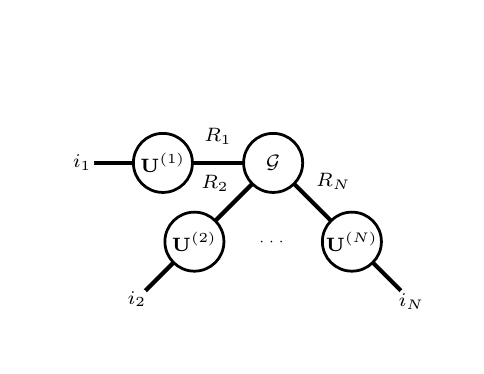
\begin{tikzpicture}[baseline={([yshift=-.5ex]current bounding box.center)}]
        \Vertex[color=white, size=0.75, label=$\mathcal{G}$]{A}
        % \draw (A) ++(-0.25,-0.25) -- ++(0.5,0.5); % Adjust the line as needed

        \Vertex[x=-1.4, color=white, size=0.75, label=$\mathbf{U}^{(1)}$]{B}
        \Vertex[x=-1, y=-1, color=white, size=0.75, label=$\mathbf{U}^{(2)}$]{C}
        \Vertex[x=1, y=-1, color=white, size=0.75, label=$\mathbf{U}^{(N)}$]{D}
        \Text[x=0.0, y=-1., fontsize=\tiny]{$\cdots$}

        \Vertex[y=-1.4, Pseudo]{Z}

        \Edge[label=$R_{1}$, position={above=1mm},color=black](A)(B)
        \Edge[label=$R_{2}$, position={above left=1mm}, color=black](A)(C)
        \Edge[label=$R_{N}$, position={above right=1mm},color=black](A)(D)

        \Vertex[x=-2.8, Pseudo]{BB}
        \Vertex[x=-2, y=-2, Pseudo]{CC}
        \Vertex[x=2, y=-2, Pseudo]{DD}

        \Edge[label=$i_1$, position={left=1mm}, color=black](B)(BB)
        \Edge[label=$i_2$, position={below left=1mm}, color=black](C)(CC)
        \Edge[label=$i_N$, position={below right=1mm}, color=black](D)(DD)

        \Vertex[y=1.4, Pseudo]{ZZ}
    \end{tikzpicture}
    \label{fig:tnd_tucker_decomposition}
\end{equation}

\begin{equation}
    \centering
    \begin{tikzpicture}[baseline={-0.5*height("$=$")}]
        \Vertex[color=white, label=$\mathcal{X}$]{A}

        \Vertex[x=-1.4, Pseudo]{C}
        \Vertex[x=-1, y=-1, Pseudo]{D}
        \Vertex[y=-1.4, Pseudo]{Z}
        \Vertex[x=1, y=-1, Pseudo]{E}
        \Vertex[x=1, y=1, Pseudo]{F}

        \Edge[label=$i_1$, position={left=1mm}, color=black](A)(C)
        \Edge[label=$i_2$, position={below left=1mm}, color=black](A)(D)
        \Text[x=0.0, y=-0.5, fontsize=\tiny]{$\cdots$}
        \Edge[label=$i_N$, position={below right=1mm}, color=black](A)(E)
    \end{tikzpicture}
    \approx \quad
    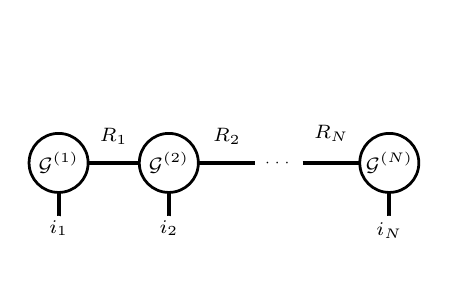
\begin{tikzpicture}[baseline={([yshift=-.5ex]current bounding box.center)}]

        \Vertex[color=white, size=0.75, label=$\mathcal{G}^{(1)}$]{A}
        \Vertex[x=1.4, color=white, size=0.75, label=$\mathcal{G}^{(2)}$]{B}
        \Vertex[x=2.8, Pseudo]{C}
        \Text[x=2.8, fontsize=\tiny]{$\cdots$}
        \Vertex[x=4.2, color=white, size=0.75, label=$\mathcal{G}^{(N)}$]{D}

        \Edge[label=$R_{1}$, position={above=1mm},color=black](A)(B)
        \Edge[label=$R_{2}$, position={above=1mm}, color=black](B)(C)
        \Edge[label=$R_{N}$, position={above=1mm},color=black](C)(D)

        \Vertex[x=0, y=-1, Pseudo]{AA}
        \Vertex[x=1.4, y=-1, Pseudo]{BB}
        \Vertex[x=4.2, y=-1, Pseudo]{DD}

        \Edge[label=$i_1$, position={below=1mm}, color=black](A)(AA)
        \Edge[label=$i_2$, position={below=1mm}, color=black](B)(BB)
        \Edge[label=$i_N$, position={below=1mm}, color=black](D)(DD)

        \Vertex[y=1.4, Pseudo]{ZZ}
    \end{tikzpicture}
    \label{fig:tnd_tt_decomposition}
\end{equation}

\begin{equation}
    \centering
    \begin{tikzpicture}[baseline={-0.5*height("$=$")}]
        \Vertex[color=white, label=$\mathcal{X}$]{A}

        \Vertex[x=-1.4, Pseudo]{C}
        \Vertex[x=-1, y=-1, Pseudo]{D}
        \Vertex[y=-1.4, Pseudo]{Z}
        \Vertex[x=1, y=-1, Pseudo]{E}
        \Vertex[x=1, y=1, Pseudo]{F}

        \Edge[label=$i_1$, position={left=1mm}, color=black](A)(C)
        \Edge[label=$i_2$, position={below left=1mm}, color=black](A)(D)
        \Text[x=0.0, y=-0.5, fontsize=\tiny]{$\cdots$}
        \Edge[label=$i_N$, position={below right=1mm}, color=black](A)(E)
    \end{tikzpicture}
    \approx \quad
    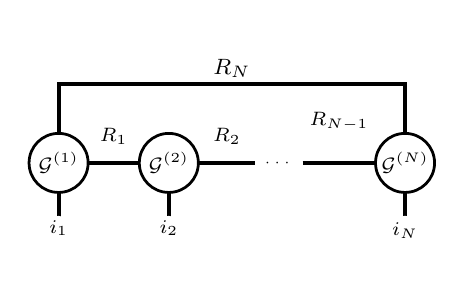
\begin{tikzpicture}[baseline={([yshift=-.5ex]current bounding box.center)}]

        \Vertex[color=white, size=0.75, label=$\mathcal{G}^{(1)}$]{A}
        \Vertex[x=1.4, color=white, size=0.75, label=$\mathcal{G}^{(2)}$]{B}
        \Vertex[x=2.8, Pseudo]{C}
        \Text[x=2.8, fontsize=\tiny]{$\cdots$}
        \Vertex[x=4.4, color=white, size=0.75, label=$\mathcal{G}^{(N)}$]{D}

        \Edge[label=$R_{1}$, position={above=1mm},color=black](A)(B)
        \Edge[label=$R_{2}$, position={above=1mm}, color=black](B)(C)
        \Edge[label=$R_{N-1}$, position={above=1mm}, color=black](C)(D)
        \Edge[path={{4.4, 1.}, {0., 1.}},color=black](D)(A)
        \Text[x=2.2, y=1.2, fontsize=\smaller]{$R_{N}$}

        \Vertex[x=0, y=-1, Pseudo]{AA}
        \Vertex[x=1.4, y=-1, Pseudo]{BB}
        \Vertex[x=4.4, y=-1, Pseudo]{DD}

        \Edge[label=$i_1$, position={below=1mm}, color=black](A)(AA)
        \Edge[label=$i_2$, position={below=1mm}, color=black](B)(BB)
        \Edge[label=$i_N$, position={below=1mm}, color=black](D)(DD)


        \Vertex[y=1.4, Pseudo]{ZZ}
    \end{tikzpicture}
    \label{fig:tnd_tr_decomposition_in_tt_format}
\end{equation}

\begin{equation}
    \centering
    \begin{tikzpicture}[baseline={-0.5*height("$=$")}]
        \Vertex[color=white, label=$\mathcal{X}$]{A}

        \Vertex[x=-1.4, Pseudo]{C}
        \Vertex[x=-1, y=-1, Pseudo]{D}
        \Vertex[y=-1.4, Pseudo]{Z}
        \Vertex[x=1, y=-1, Pseudo]{E}
        \Vertex[x=1, y=1, Pseudo]{F}

        \Edge[label=$i_1$, position={left=1mm}, color=black](A)(C)
        \Edge[label=$i_2$, position={below left=1mm}, color=black](A)(D)
        \Text[x=0.0, y=-0.5, fontsize=\tiny]{$\cdots$}
        \Edge[label=$i_N$, position={below right=1mm}, color=black](A)(E)
    \end{tikzpicture}
    \approx
    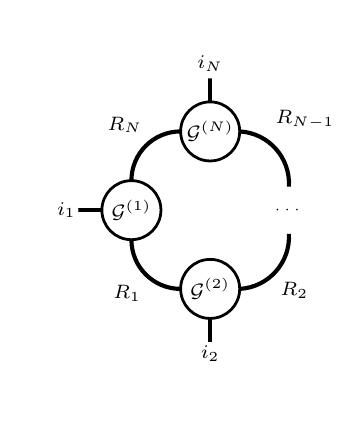
\begin{tikzpicture}[baseline={([yshift=-.5ex]current bounding box.center)}]



        \Vertex[x=-1., color=white, size=0.75, label=$\mathcal{G}^{(1)}$]{A}
        \Vertex[y=-1., color=white, size=0.75, label=$\mathcal{G}^{(2)}$]{B}
        \Vertex[x=1., Pseudo]{C}
        \Text[x=1., fontsize=\tiny]{$\cdots$}
        \Vertex[y=1., color=white, size=0.75, label=$\mathcal{G}^{(N)}$]{D}

        \Edge[label=$R_{1}$, bend=-45, position={below left=1mm},color=black](A)(B)
        \Edge[label=$R_{2}$, bend=-45, position={below right=1mm}, color=black](B)(C)
        \Edge[label=$R_{N-1}$, bend=-45, position={above right=1mm},color=black](C)(D)
        \Edge[label=$R_{N}$, bend=-45, position={above left=1mm},color=black](D)(A)

        \Vertex[x=-2., Pseudo]{AA}
        \Vertex[y=-2., Pseudo]{BB}
        \Vertex[y=2., Pseudo]{DD}

        \Edge[label=$i_1$, position={left=1mm}, color=black](A)(AA)
        \Edge[label=$i_2$, position={below=1mm}, color=black](B)(BB)
        \Edge[label=$i_N$, position={above=1mm}, color=black](D)(DD)

        \Vertex[y=1.4, Pseudo]{ZZ}
    \end{tikzpicture}
    \label{fig:tnd_tr_decomposition}
\end{equation}


\end{document}